\documentclass[]{article}

\usepackage[utf8]{inputenc}
\usepackage[russian]{babel}
\usepackage[left=1.5cm,right=1.5cm,top=2cm,bottom=2.5cm]{geometry}

\usepackage[fontsize=13pt]{scrextend}

% что-то за межстрочный интервал отвечающее
\renewcommand{\baselinestretch}{1.3}

\usepackage[nooneline]{caption}
\usepackage{subcaption}
\usepackage{indentfirst}
\usepackage{tabularx}
\usepackage{amsmath}
\usepackage{multirow}
\usepackage{hyperref}



\usepackage{fancyhdr}


\setlength{\headheight}{15mm}


\usepackage[pdftex]{graphicx}
\graphicspath{{/home/maxim/Projects/Vega/Finance Econometrics/Project2/Report/img}}

\pagestyle{fancy}
\lhead{\textbf{\normalsize Проект 2}}
\rhead{\textbf{\normalsize Выполнили: }\normalsize Кирякин Максим, Куренкова Дарья, Коваль Наталия}



\begin{document}

{
	\Large
	\href{https://github.com/MaximKiryakin/Vega/tree/FinanceEconometrics/Project2}{Репозиторий проекта}.
}

\section{Постановка задачи}


В работе было необходимо построить прогнозы для волатильности выбранного актива с использованием GARCH и HAR моделей. 

[Bollerslev, 1986]: \textbf{GARCH(p, q)} модель:

$$\varepsilon_t = \nu_t \sqrt{h_t}$$
$$h_t = a_0 + a_1\varepsilon_{t-1}^2 + ... + a_p\varepsilon_{t-p}^2 + b_1 h_{t-1} + ... + b_q h_{t-q}$$

где: $\nu_t \sim iid$, $\mathbf{E}(\nu_t) = 0$, $\mathbf{D}(\nu_t) = 1$, $a$, $b$ -- параметры.

\textbf{Реализованная волатильность}

$RV_t$ -- реализованная волатильность для периода $t$ (обычно день) задается следующей формулой:

$$RV_{t} = \sqrt{\sum_{j}r_{t, j}^2}$$


где: $r_{t, j} = \log{p_{t, j}} - \log{p_{t, j-1}}$ -- лог. доходность для периода $j$ дня $t$; $p_{t, j}$ -- цена актива в день $t$ во внутренний период $j$.


[Corsi, 2009]: \textbf{HAR(w, m)} модель: 

$$RV_t = \beta_0 + \beta_1 RV_{t-1} ++ \beta_2 RV_{t-1}^w + \beta_3 RV_{t-1}^m + \varepsilon_t$$

где: 

$RV_{t}^w = \frac{1}{w}\sum_{j=0}^{w-1}RV_{t-j}$ -- средняя реализованная волатильность за неделю; 
$RV_{t}^m = \frac{1}{m}\sum_{j=0}^{m-1}RV_{t-j}$ -- средняя реализованная волатильность за месяц; $w$ -- число торговых дней в неделе; $m$ -- число торговых дней в месяце.



\section{Данные}


В качестве базового актива рассматривались котировки акций Сбербанка с 3-ого января 2020 года по 29 ноября 2024 года.  Сбербанк (Тикер SBER) -- российский финансовый конгломерат, крупнейший универсальный банк России и Восточной Европы. Акции банка торгуются на московской биржи, входят в список <<голубых фишек>> российского фондового рынка и хорошо отражают его динамику ($\beta = 0.82$ на 1 декабря 2024).

Проект был выполнен с использованием двух языков: Python и R. Первый использовался для первичной обработки и анализа данных котировок, второй -- для построения и оценки моделей.
Данные были загружены с помощью функции getSymbols пакета rusquant языка R. Частотность данных -- 5 минут.
Итоговый датафрейм содержал 95868 записей. На рисунках $\ref{price}$ и $\ref{vol}$ представлены цены акции Сбера за указанный промежуток и ее доходность соответственно.

\begin{figure}[h!]
	\centering
	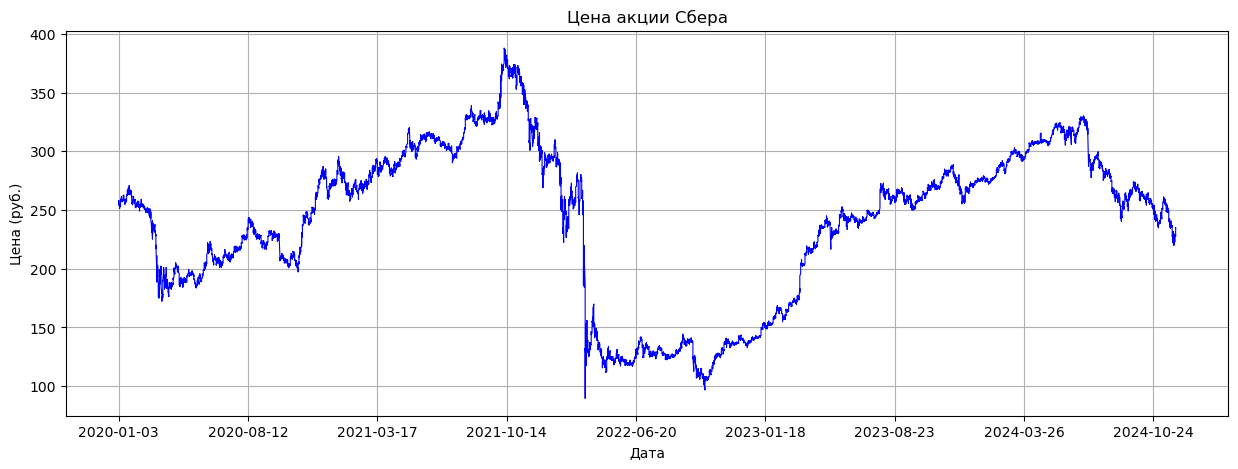
\includegraphics[width=1.\textwidth]{price.png}
	\caption{Цена акции Сбера на момент закрытия за промежуток 2020-01-03 2024-11-28.}
	\label{price}
\end{figure}

\begin{figure}[h!]
	\centering
	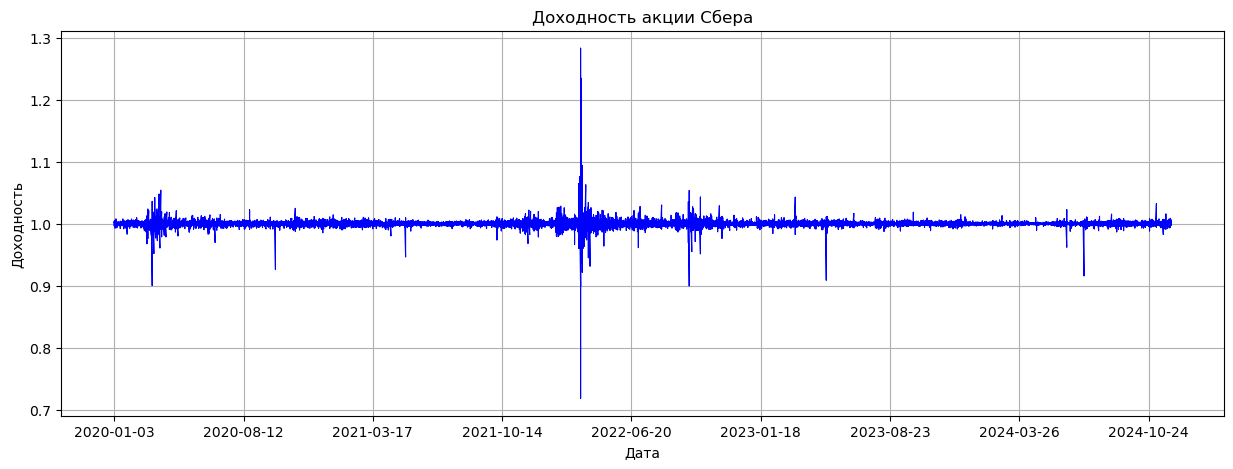
\includegraphics[width=1.\textwidth]{vol.png}
	\caption{Динамика доходности акции Сбера за промежуток 2020-01-03 2024-11-28.}
	\label{vol}
\end{figure}

Из рисунка $\ref{vol}$ видно, что в данных присутствует кластеризация волатильности. Помимо этого также были выявлены пропуски в данных для тех дней, в которые не было торгов. При обучении моделей эти периоды были исключены.

Кроме того, на рисунке $\ref{hist}$ представлена гистограмма для доходностей, для которой выполнена ядерная оценка плотности. Для сравнения на рисунок также добавлена плотность нормального распределения. Из графика видно, что реальная оценка плотности отличается от нормальной. Исходя из этих распределений, можно предположить, что модели, с нормальным распределением остатков остатков будут работать хуже, чем те, у которых предполагается, например, распределение Стьюдента. 

\begin{figure}[h!]
	\centering
	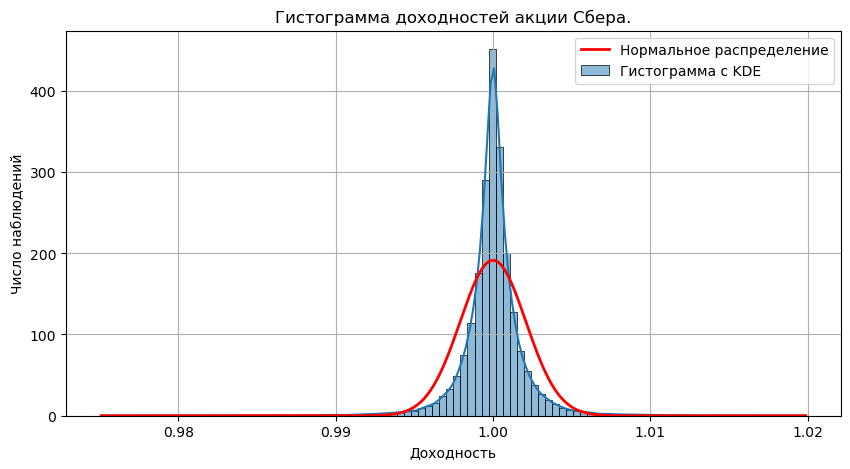
\includegraphics[width=1.\textwidth]{hist.png}
	\caption{Гистограмма доходностей акции Сбера за промежуток 2020-01-03 2024-11-28.}
	\label{hist}
\end{figure}




\section{Ход работы}
\subsection{Выбранные модели и их спецификация}


В сравнении участвуют следующие пять GARCH-моделей.

1. Стандартный GARCH(p, q)
$$\varepsilon_t = \nu_t \sqrt{h_t}$$
$$h_t = a_0 + a_1\varepsilon_{t-1}^2 + ... + a_p\varepsilon_{t-p}^2 + b_1 h_{t-1} + ... + b_q h_{t-q}$$

здесь и далее: $h_t$ — условная дисперсия в момент $t$; $a$, $b$ — параметры, оцениваемые методом максимального правдоподобия; $\nu_t \sim iid$, $\mathbf{E}(\nu_t) = 0$, $\mathbf{D}(\nu_t) = 1$; $a$, $b$ -- параметры.

2. Экспоненциальный GARCH (EGARCH)
$$\ln{h_t} = a_0 + a_1(|\varepsilon_{t-1}| - E(|\varepsilon_{t-1}|)|) + \theta\varepsilon_{t-1} + b\ln{h_{t-1}}$$

3. Интегрированный GARCH (iGARCH)

Накладывается дополнительное условие на коэффициенты:

$$\sum_{i=1}^{p} a_i + \sum_{i=1}^{q} b_i = 1$$

4. Пороговый GARCH (TGARCH)
$$\sqrt{h_t} = a_0 + a_1^{+}\varepsilon_{t-1}^{+} + a_1^{-}\varepsilon_{t-1}^{-} + b_1\sqrt{h_{t-1}}$$

$$
	\varepsilon_{t-1}^{+} =
	\begin{cases}
		\varepsilon_{t-1}, & \text{если} \ \varepsilon_{t-1} > 0 \\
		0, & \text{иначе}
	\end{cases}
$$

$$
	\varepsilon_{t-1}^{-} =
	\begin{cases}
		\varepsilon_{t-1}, & \text{если} \ \varepsilon_{t-1} < 0 \\
		0, & \text{иначе}
	\end{cases}
$$

5. Нелинейный/ассиметричный NAGARCH
$$h_t = a_0 + a_1(\varepsilon_{t-1} - \theta\sqrt{h_{t-1}})^2 + b_1 h_{t-1}, \theta > 0$$


Каждая из выше перечисленных моделей GARCH-типа оценивается с каждой из трех моделей условного распределения ошибок:

1. Стандартное нормальное распределение (norm) с функцией плотности

\begin{equation}
	\varphi(x) = \frac{1}{\sqrt{2\pi}} e^{-\frac{x^2}{2}}.
\end{equation}

2. Скошенное нормальное распределение (snorm)

\begin{equation}
	f(x) = 2\varphi(x)\Phi(\alpha x),
\end{equation}

где \(\varphi(x)\) и \(\Phi(x)\) — функция плотности вероятности и функция распределения стандартной нормальной случайной величины.

3. Скошенное \(t\)-распределение Стьюдента (\textit{sstd}) 

$$f(z, \xi) = \frac{2}{\xi + \xi^{-1}} \left[ f(\xi z) I(-z) + f(z/\xi) I(z) \right]$$

где \(f(x)\) плотность распределения Стьюдента
$$I(z) = 
\begin{cases} 
	1, & z > 0, \\
	0, & z \leq 0. 
\end{cases}
$$

Помимо моделей семейства GARCH были рассмотрены так же следующие три HAR модели:

1. HAR модель

$$RV_t = \beta_0 + \beta_1 RV_{t-1} ++ \beta_2 RV_{t-1}^w + \beta_3 RV_{t-1}^m + \varepsilon_t$$

где:
\begin{itemize}
	
	\item $RV_t$ -- реализованная волатильность для периода $t$
	
	\item $r_{t, j} = \log{p_{t, j}} - \log{p_{t, j-1}}$ -- лог. доходность для периода $j$ дня $t$
	
	\item $RV_{t} = \sqrt{\sum_{j}r_{t, j}^2}$ 
	
	\item $RV_{t}^w = \frac{1}{w}\sum_{j=0}^{w-1}RV_{t-j}$
	
	\item $RV_{t}^m = \frac{1}{m}\sum_{j=0}^{m-1}RV_{t-j}$
	
\end{itemize}

2. HARQ модель:
$$RV_t = \beta_0 + \beta_1 RV_{t-1} + \beta_2 RV_{t-1}^w + \beta_3 RV_{t-1}^m + \beta_{1Q}\sqrt{RQ_{t-1}}RV_{t-1} + \beta_{2Q}\sqrt{RQ_{t-1}^w} RV_{t-1}^w  + \beta_{3Q}\sqrt{RQ_{t-1}^m}RV_{t-1}^m + \varepsilon_{t}$$

где: $RV_t$ -- реализованная волатильность для периода $t$; $r_{t, j} = \log{p_{t, j}} - \log{p_{t, j-1}}$ -- лог. доходность для периода $j$ дня $t$; $RV_{t} = \sqrt{\sum_{j}r_{t, j}^2}$; $RV_{t}^w = \frac{1}{w}\sum_{j=0}^{w-1}RV_{t-j}$; $RV_{t}^m = \frac{1}{m}\sum_{j=0}^{m-1}RV_{t-j}$; $RQ_{t} = \sum_{j=0}r_{tj}^4$	-- realised quartisity.

3. HARJ модель:

$$RV_t = \beta_0 + \beta_1 RV_{t-1} + \beta_2 RV_{t-1}^w + \beta_3 RV_{t-1}^m + \beta_{4}J_t + \beta_5 J_t^w + \beta_6 J_t^m + \varepsilon_{t}$$

где:

$BPV_t == \sum_{j=1}r_{t, j}r_{t, j-1}$ -- realized bipower variation. Позволяет учитывать тренд в данных.

$Jump: J = max(RV_t - BPV_t, 0)$


\subsection{Сравнение моделей GARCH}


Модели было решено оценивать по трем метрикам: MSE, MAE, MAPE. При этом для моделей семейства GARCH в качества наивного прогноза рассматривался GARCH(1, 1)-norm. Валидация моделей проходила на значениях цен акций Сбера в интервале с 2024-20-21 по 24-11-29. Для расчета метрик использовалось расщиряющееся окно. Предсказания производились на один день вперед. В качестве целевой переменной расчитывалась реализованная волотильность в кадый из дней.
Для прогноза ипользовалась библиотека языка R rugarch.

Было установлено, что валидация модели семейства GARCH на домашнем пк занимаем более часа, что сделало невозможным валидацию на расширяющемся окне всех моделей. При этом иногда могли возникать проблемы со сходимостью методов и приходилось перезапускать основной цикл перебора моделей. При этом сокращение числа наблюдений было нецелесообразно, так как для обучения данного класса моделей число наблюдений должно 
составлять десятки тысяч.

Поэтому был предложен альтернативный подход сравнения моделей. Ранжирование моделей производилось согласно информационным критерия AIC и BIC. А лучшие модели оценивались на расширяющемся окне.




\begin{table}[h!]
	\centering
	\caption{Значения информационных критериев для различных GARCH моделей.}
	\begin{tabularx}{\textwidth}{|X|X|X|l|l|l|}
		\hline
		                    	& AIC        & BIC        & MAE          & MSE             & MAPE    \\ \hline
		GARCH(1, 1)-norm        & -9.935168  & -9.934575  & 0.02184 &  0.000488   & 0.995   \\ \hline
		TGARCH(1, 1)-sstd       & -10.36761  & -10.36682  &0.02183  &0.000487     &0.994   \\ \hline
		     ...    &  &   &&&    \\ \hline
		NAGARCH(1, 1)-norm      & -9.937876  & -9.860202  &&&    \\ \hline
		
		
	\end{tabularx}
	\label{tab:1}
\end{table}



Эксперименты показали, что, как и ожидалось, скошенное распределение Стьюдента показывает лучшие значения для информационных критериев, чем остальные распределения. Графики QQ-plot для нормального и скошенного распределений приведены на рисунках $\ref{badQQ}$ и $\ref{goodQQ}$ соответственно.


\begin{figure}[h!]
	\centering
	\begin{subfigure}{0.49\textwidth}
		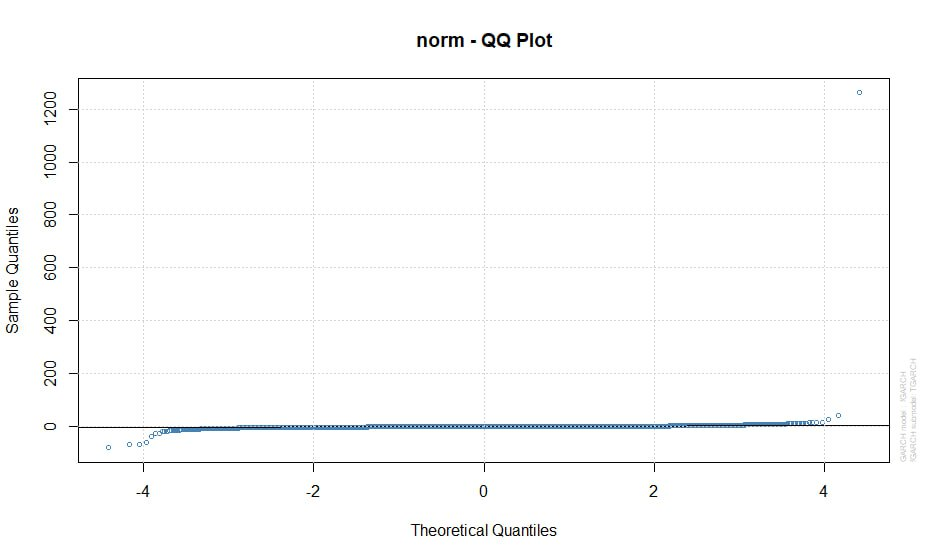
\includegraphics[width=\linewidth]{badQQ.jpg}
		\caption{QQ-plot для модели TGARCH (нормальное распределение ошибки).}
		\label{badQQ}
	\end{subfigure}
	\hfill
	\begin{subfigure}{0.49\textwidth}
		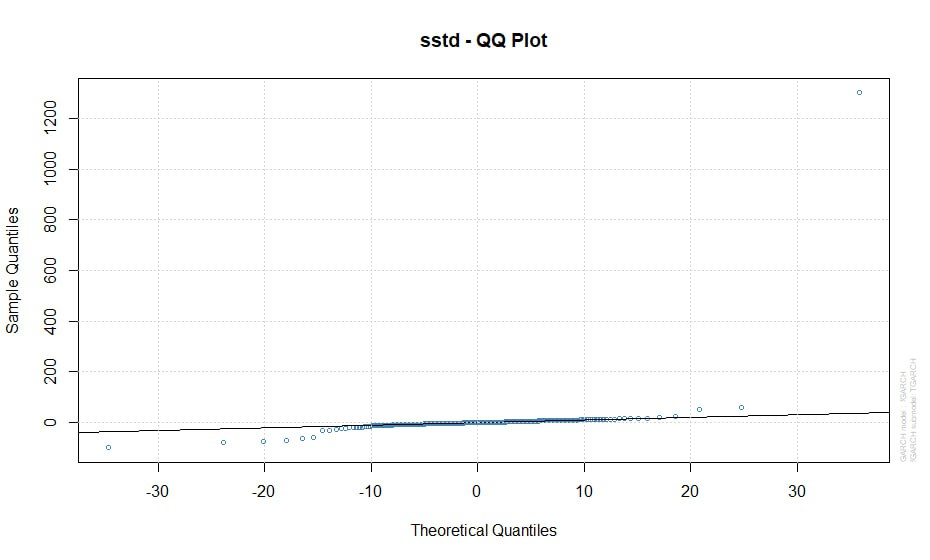
\includegraphics[width=\linewidth]{goodQQ.jpg}
		\caption{QQ-plot для модели TGARCH (скошенное распределение Стьюдента ошибки).}
		\label{goodQQ}
	\end{subfigure}
\end{figure}




Также на рисунках $\ref{normNews}$ и $\ref{skewNews}$ приведены графики влияния типа новостей на волатильность. Видно, что для TGARCH это график несимметричен, что говорит о том, что негативные новости влияют на волатильность сильнее, чем позитивные.

\begin{figure}[h!]
	\centering
	\begin{subfigure}{0.49\textwidth}
		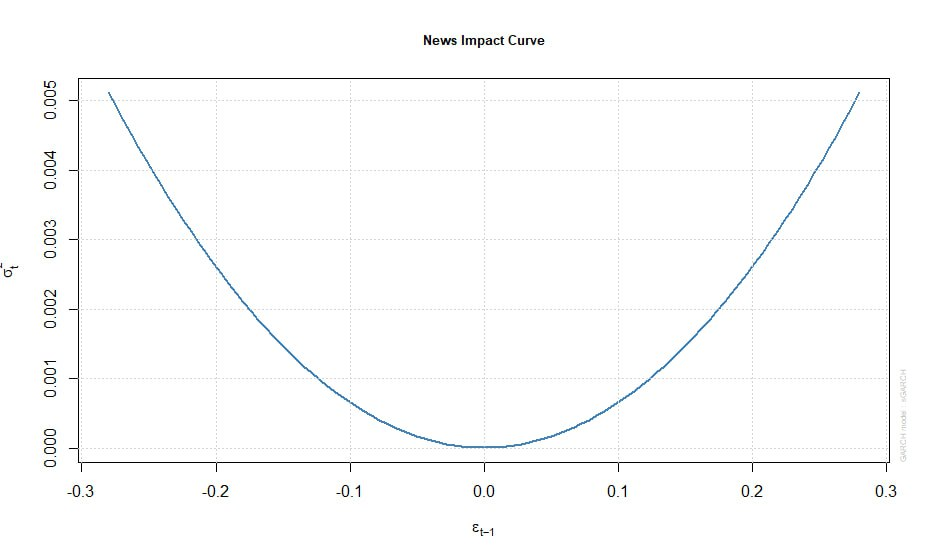
\includegraphics[width=\linewidth]{normNews.jpg}
		\caption{Влияние положительных и отрицательных новостей на волатильность для GARCH.}
		\label{normNews}
	\end{subfigure}
	\hfill
	\begin{subfigure}{0.49\textwidth}
		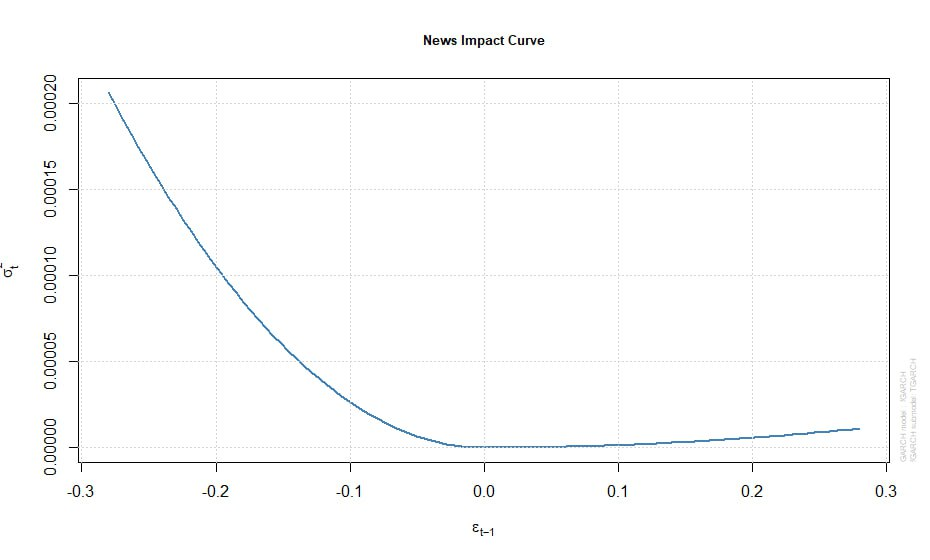
\includegraphics[width=\linewidth]{skewNews.jpg}
		\caption{Влияние положительных и отрицательных новостей на волатильность для TGARCH.}
		\label{skewNews}
	\end{subfigure}
	\label{fig:both_images}
\end{figure}

В ходе экспериментов также было установлено, что из-за того, что модель плохо отлавливает динамику волатильности на один день вперед (в нашем случае это больше 100 пятиминутных интервалов), все результаты оказались примерно похожими. Для того, чтобы провести эксперимент с прогнозированием на каждом шаге на 5 минут вперед нужен суперкомпьютер. Но и точность прогноза тогда должна существенно увеличиться. Из таблицы $\ref{tab:1}$ видно, что лучшей моделью с точки зрения информационных критериев оказалась TGARCH(1,1) -sstd, но ее преимущество относительно наивного прогноза GARCH(1, 1)-norm совсем незначительно при валидации на расширяющемся окне.


\subsection{Сравнение моделей HAR}

Для прогнозов HAR модели использовались те же данные, что и для GARCH моделей. Прогноз осуществлялся на тот же горизонт, что позволяет сравнить эти два подхода. Для построения прогноза использовалась функция библиотеки HARModel: HARForecast. Результаты работы HAR моделей приведены в таблице $\ref{tab:2}$. Можно видеть, что лучше всего на выбранном валидационном интервале себя показала простая HAR модель.

\begin{table}[h!]
	\centering
	\caption{Значения метрик для различных HAR моделей.}
	\begin{tabularx}{\textwidth}{|X|X|X|X|}
		\hline
		       &   MAE        & MSE       & MAPE    \\ \hline
		HAR    & 0.002981667  & 1.768148e-05  & 0.198    \\ \hline
		HARQ   & 0.004232569  & 3.178277e-05  & 0.286    \\ \hline
		HARJ   & 0.003746625  & 2.624049e-05  & 0.253    \\ \hline
	\end{tabularx}
	\label{tab:2}
\end{table}

На рисунках $\ref{HAR}$ и $\ref{HARQ}$ представлены прогнозы волатильности на 30 дней вперед для HAR и HARQ моделей соответственно.


\begin{figure}[h!]
	\centering
	\begin{subfigure}{0.49\textwidth}
		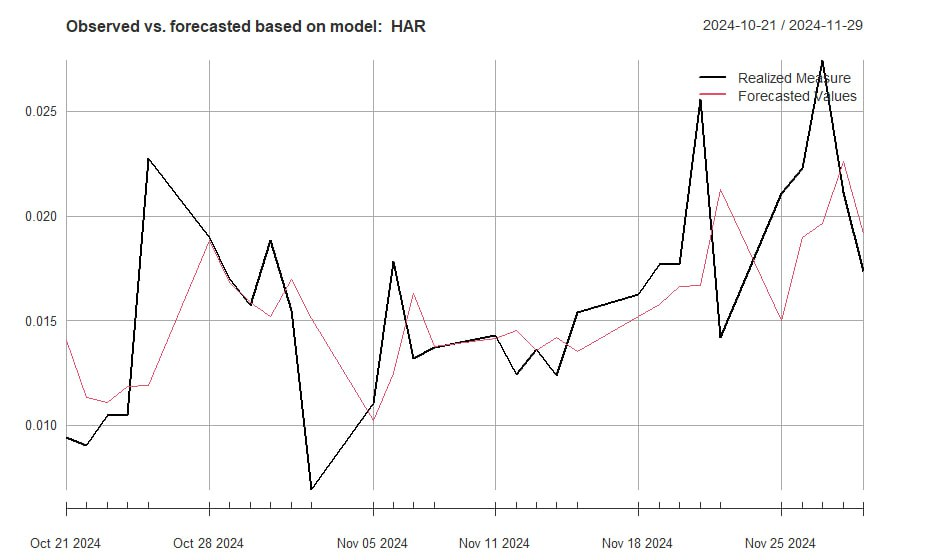
\includegraphics[width=\linewidth]{HAR.jpg}
		\caption{Прогноз волатильности HAR моделью на 30 дней.}
		\label{HAR}
	\end{subfigure}
	\hfill
	\begin{subfigure}{0.49\textwidth}
		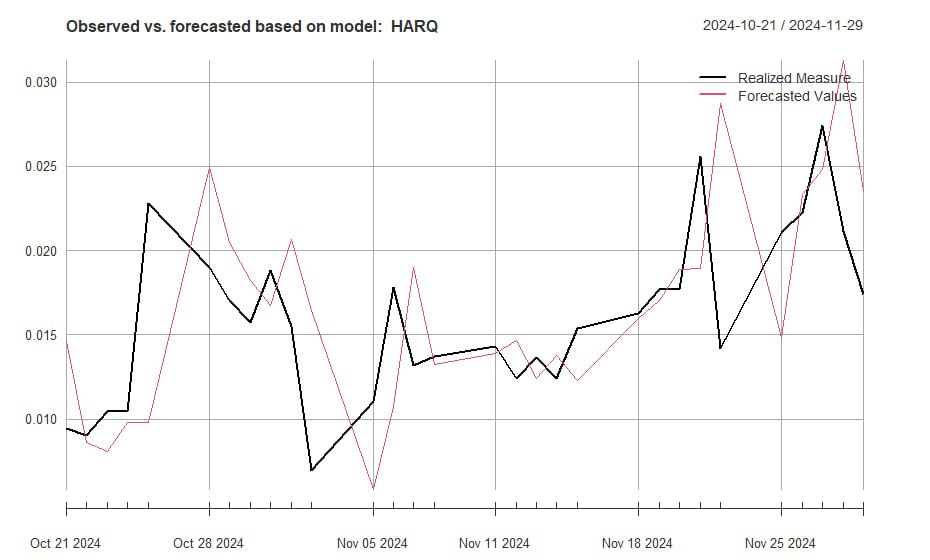
\includegraphics[width=\linewidth]{HARQ.jpg}
		\caption{Прогноз волатильности HARQ моделью на 30 дней.}
		\label{HARQ}
	\end{subfigure}
	\label{fig:both_images}
\end{figure}


\subsection{Сравнение моделей HAR на данных повышенной волатильности}

Помимо изменения спецификаций моделей в работе было решено также протестировать модели на разных временных промежутках. В качестве второго временного интервала рассматривались даты с 1 января 2017 по 25 марта 2020. В этот период российский фондовый рынок был крайне нестабилен всвязи с распространением COVID. 

Для тестов было решено использовать HAR модели, так как они показали результаты лучше, чем GARCH модели при первичном тестировании. Кроме того, скорость их обучения на порядок выше, что было очень существенно для нас. Прогноз также выполнялся с помощью расширяющегося окна. Сам прогноз строился на 1 день вперед. Результаты работы алгоритмов приведены в таблице $\ref{tab:3}$.


\begin{table}[h!]
	\centering
	\caption{Значения метрик для различных HAR моделей на данных повышенной волатильности.}
	\begin{tabularx}{\textwidth}{|X|X|X|X|}
		\hline
		       &   MAE   & MSE      & MAPE     \\ \hline
		HAR    & 0.0088  & 0.00018  & 0.300    \\ \hline
		HARQ   & 0.0090  & 0.00019  & 0.305    \\ \hline
		HARJ   & 0.0099  & 0.00021  & 0.324    \\ \hline
	\end{tabularx}
	\label{tab:3}
\end{table}

Из таблицы видно, что на волатильных данных прогнозы HAR и HARQ очень близки $\frac{MAE(HARQ)}{MAE(HAR)} = 1.034841)$. Что не позволяет абсолютно точно сказать, что первая из моделей лучше и требует более детальных тестов.

На рисунках $\ref{HARVol}$, $\ref{HARQVol}$ приведены графики прогнозов моделей HAR и HARQ на волатильных данных. 


\begin{figure}[h!]
	\centering
	\begin{subfigure}{0.49\textwidth}
		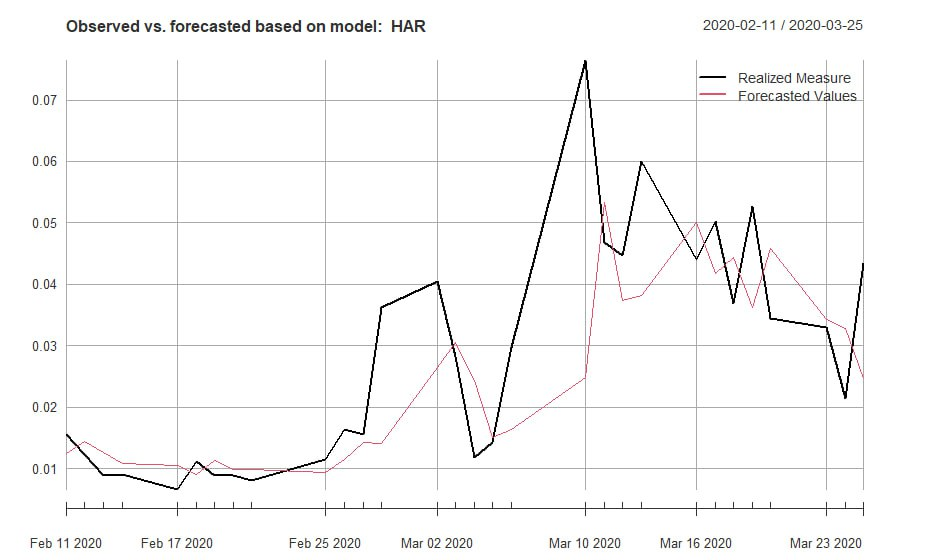
\includegraphics[width=\linewidth]{HARVol.jpg}
		\caption{Прогноз HAR моделью на волатильных данных.}
		\label{HARVol}
	\end{subfigure}
	\hfill
	\begin{subfigure}{0.49\textwidth}
		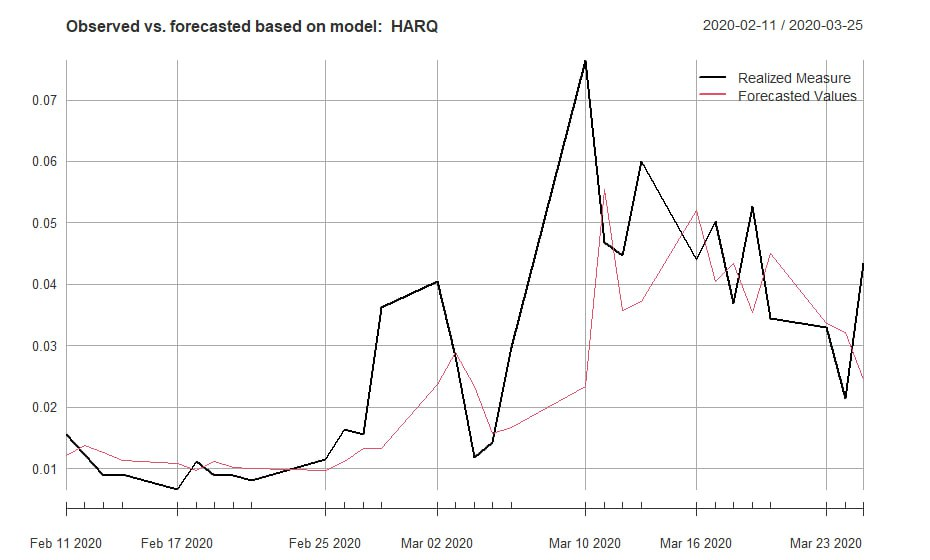
\includegraphics[width=\linewidth]{HARQVol.jpg}
		\caption{Прогноз HARQ моделью на на волатильных данных.}
		\label{HARQVol}
	\end{subfigure}
\end{figure}


\section{Заключение}

В работе проводилось сравнение двух классов моделей предсказания волатильности HAR и GARCH. В качестве базового актива были выбраны акции Сбера. Всего рассматривалось два временных интервала: с 3-ого января 2020 года по 29 ноября 2024 года и с 1 января 2017 по 25 марта 2020. Причем второй интервал рассматривался только для HAR моделей и считался более волатильным, чем первый.

В сравнении участвовали следующие модели семейства GARCH: GARCH, EGARCH, NAGARCH, TGARCH, IGARCH. И следующие модели семейства HAR: HAR, HARQ, HARJ.
На первом наборе данных среди GARCH моделей лучше всего себя показал TGARCH(1, 1)-sstd, а из семейства HAR -- обычная HAR модель. Притом на высоковолатильных данных результаты HAR и HARQ сопоставимы. Результаты работы отобранных алгоритмов приведены в таблице $\ref{tab:4}$.

\begin{table}[h!]
	\centering
	\caption{Значения метрик отобранных моделей предсказания волатильности.}
	\begin{tabularx}{\textwidth}{|X|X|X|X|l|}
		\hline
								  & Модель           &   MAE   & MSE     & MAPE     \\ \hline
		                          & TGARCH(1,1)-sstd & $2.2\cdot10^{-2}$ & $4.9\cdot10^{-4}$  & 0.994    \\ \cline{2-5}
		\centering{Период}        & GARCH(1,1)-norm  & $2.2\cdot10^{-2}$ & $4.9\cdot10^{-4}$  & 0.995    \\ \cline{2-5}
    	\centering{c 03-01-2020}  & HAR              & $3.0\cdot10^{-3}$ & $1.8\cdot10^{-5}$  & 0.198    \\ \cline{2-5}
    	\centering{по 29-11-2024} & HARQ             & $4.2\cdot10^{-3}$ & $3.2\cdot10^{-5}$  & 0.286    \\ \cline{2-5}
    	                          & HARJ             & $3.7\cdot10^{-3}$ & $2.6\cdot10^{-5}$  & 0.253    \\ \cline{2-5}
    	                          & Naive            & $3.3\cdot10^{-3}$ & $2.7\cdot10^{-5}$  & 0.221    \\ \hline
		\centering{Период}        & HAR              & $8.8\cdot10^{-3}$ & $1.8\cdot10^{-4}$  & 0.300    \\ \cline{2-5}
		\centering{c 01-01-2017}  & HARQ             & $9.0\cdot10^{-3}$ & $1.9\cdot10^{-4}$  & 0.305    \\ \cline{2-5}
		\centering{по 25-03-2020} & HARJ             & $9.9\cdot10^{-3}$ & $2.1\cdot10^{-4}$  & 0.324    \\ \cline{2-5}
		                   & Naive            & $1.4\cdot10^{-2}$ & $3.3\cdot10^{-4}$  & 0.868    \\ \cline{2-5}
		\hline
	\end{tabularx}
	\label{tab:4}
\end{table}

В результате экспериментов было установлено, что прогноз HAR моделей является гораздо более точным по сравнению с GARCH. Однако качество модели GARCH может быть улучшено, если делать прогноз не на день, а, например, на 5 мин вперед.

Кроме того, в таблицу также добавлены значения метрик наивного прогноза реализованной волатильности, в качестве которого бралось среднее значение за последние 3 дня. Эксперименты показывают, что для относительно неволатильных данных наивный прогноз даже превзошел HAR модели по метрике MAPE. При этом на волатильных данных наивный прогноз проигрывает HAR моделям. На основании этих результатов можно говорить об эффективности HAR моделей на волатильных данных.

Также за время написани данного проекта его авторами были с нуля изучены основы языка R.

\end{document}
